\documentclass{article}
\setlength\parindent{0pt}
\usepackage[hmargin=1in,vmargin=1in]{geometry}
\usepackage{cmll}
\usepackage{amsmath}
\setlength{\parskip}{.5em}
\usepackage{graphicx}

\title{CMPT 409 Assignment 6}
\author{Heather Li, Ekjot Singh Billing, Manshant Singh Kohli}

\begin{document}
\maketitle

\section{Bejeweled Help}
Given the small scope of this problem, a brute force solution will suffice.
\par 
Consider all the possible swaps that could occur. First consider the horizontal swaps. All swaps must be between adjacent jewels so in each row, there are 7 possible swaps. There are 8 rows, so there are 56 horizontal swaps. Similarly, there are 56 possible vertical swaps. As there are only 112 gem swaps in total, we can simply try all possible swaps. Note that the board does not contain three-in-a-row/column gems, so the maximum size of a in-a-row/column configuration is 5 gems
\par
Store our representation of the board in an 8x8 array. Store each possible swap in two 8x7 arrays (for each swap orientation).  For each row and column, we consider what would happen if we swap adjacent jewels. After each possible swap, we can consider the 5x5 grid around the swap and determine whether either of the swapped gems has created a scorable configuration. We store the points in an array.
\par 
After iterating through every swap, we return the largest values from our swap arrays, in addition to the indices where they were found (the swaps which created them).


\section{Binary}
Partition our binary sequence based on the binary numbers represented in each partition. The $m$th partition should contain all the binary numbers which take exactly $m$ digits to represent. (Except for the 0th partition, which contains '0' and the 1st partition, which consists of '1'). 
\par 
We wish to get to the partition in which the $k$th digit can be found. We do so by tracking three variables $n,m,$ and $N$. $m$ is associated with the number of binary digits that numbers in the partition take to represent. $n$ refers to the largest number represented in the sequence, before this partition. $N$ is the number of digits contained in the sequence before this partition.
\par 
(Excluding the 0th partition) We start off in the first partition with $m=1, n=0,N=0$. To advance partitions, we increment $m$ by 1, $n$ by $2^{m-1}$, and $N$ by $(2^{m-1})m$. We continue advancing partitions until we get to the partition where $N$ would be greater than $k$. We return to the previous partition, as the $k$th digit is located in it.
\par 
As each number in this partition takes $m$ digits to represent, we know that the $k$th digit will be contained in the $\lfloor (k-N)/m \rfloor$th number in this partition, or the $\lfloor (k-N)/m \rfloor + n +1$th number.
\par 
The $m-((k-N)$ mod $n))$th (least significant) digit of this number's binary representation is the $k$th digit of our sequence.
\par 
After establishing our $k,m,$ and $N$ values, we could reach the $k$th binary digit with (in C syntax):
\[( (\lfloor (k-N)/m \rfloor + n +1) >> (m-(k-N)\%m) ) \with\with   1 \]


\section{City Slickers}
First, we do a graph coloring and create disjoint sets of '.' and 'r', and keep track of the 2 groups that contain the 'r's. If both the 'r's are in the same group then the answer is 0. This can be computed in O(r*c) time.
\par
Next, we create a graph where the edges are stored in HashMap where the key is the x,y coordinates and the value is a HashSet of all the edges it connects to. I am using this since it provides me a O(1) time add and query edges of a node. I then store all the surrounding mountains in (north, south, east, west) of each mountain with the joining mountain. This can be done in another O(r*c) time.
\par
Next, for each one of the colored groups above, I create an c++ vector of mountains surrounding that group. Then I create an edge from each mountain in the vector to every other mountain. This can be done in another O(r*c) time.
\par
Now all that is left is to create a simple BFS graph traversal from one group with 'r' to another since the HashMap contains the edges for immediate reachable mountains and the minimum route represents the minimum number mountains that are needed to be crosed to reach the destination. For this we can do this iteratively by using a Queue, and a HashSet. Queue will contain the next coordinates to visit and the minimum number steps needed to get to these coordinates. HashSet will contain where mountain at this coordinates has been visited during the BFS treversal before or not. This BFS will take another O(r*c) time.
\par
So the total algorithm will take O(r*c) time

\section{Cutting Pizza}
As all 12 outer pieces of the pizza must be the same size, all 3 outer pieces contained in a quarter of the pizza must be the same size, and all quarters of the pizza must have pieces of the same size. It is sufficient to consider a quarter of the pizza.
\par
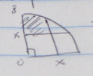
\includegraphics{pizzadiagram}
\par
We wish to determine the area of the shaded region as a function of $x$.
\[A(x)=\int^x_0{\sqrt{64-x^2}dx}-x^2\]
\[=(\frac{x}{2}\sqrt{64-x^2}+32\arcsin(\frac{x}{8}))| ^x_0 -x^2\]
\[=\frac{x}{2}\sqrt{64-x^2}+32\arcsin(\frac{x}{8}) -x^2\]
\par 
The area of a quarter of a circle with diameter 8 is $8^2\pi/4=16\pi$. Each quarter should consist of a square of area $x^2$ and three equally sized outer regions of area $A(x)$ each.
\par 
As we must have $0 < x <8$, we can run a binary search using these parameters. We wish to have the value of $3A(x)+x^2$ be as close as possible to $16\pi$. We will continuously refine our value of $x$ until the distance between our bounds $hi$ and $lo$ is less than $0.0001$. Note that in our domain, $3A(x)+x^2$ is a decreasing function.
\par 
Initially set $lo=0$ and $hi=8$ and $mid=(hi-lo)/2$. If $3A(x)+x^2$ is less than $A(x)$ we should decrease the value of $x$ in our binary search (move $hi=mid$ and recalculate the value of $mid$).  If $3A(x)+x^2$ is greater than $A(x)$ we should increase the value of $x$ in our binary search (move $lo=mid$ and recalculate the value of $mid$). 
\par 
This will produce $x$, correct up to 4 decimal places.

\section{Doing Laundry}
The optimal time will have the dryer always running. As each load takes an equal amount of time to run and there is no limit on the size of the dryer backlog, we should run our laundry loads in order of most dryer time to least dryer time. This can be accomplished by putting the list of laundry loads in a vector and then sorting them in descending order. 
\par 
Once we have the optimal order, we can iterate through them to determine the amount of time used. We track this time in minutes with the variable $sofar$. Initialize $i=30$, as the first load must spend 30 minutes in the washer and the dryer cannot be running.
\par 
For each $i$th element in our sorted vector $v$, we check whether $30i<sofar$. If this is the case, then this means that after the $ith$ load, we must spend time waiting before we can put the $ith$ load into the dryer. In this case, we set $sofar=30i+v[i]$.
\par 
Otherwise, there is already a laundry load ready to dry when we end. In this case, we increment $sofar$ by $v[i]$.
\par 
Once we process all the laundry loads, we convert $sofar$ from minutes to an $HH:MM$ format and print it.

\section{Linking Logos}
Consider the block in the top left corner. It has length $x$. The bottom right block must not be the same length, so it must be shorter or longer. Now consider the shorter side (top or bottom). The block inserted must not be the same length as the gap. We can proceed in this fashion until either (1) one side reaches length $n$ or (2) there are no valid blocks left to insert. At each stage, there will be at most 4 blocks to consider adding.
\par 
We can use divide and conquer and only construct half the blocks. We can then store this in a map, where the key is the number of blocks we have left in a construction. If a half-construction has a corresponding (uses the blocks it doesn't) half-construction which matches up to it, then there is a valid configuration. Otherwise, there is not.

\section{Longshot}
We solve this problem recursively. Note that in a group of 16 people, there will be three matches played before players reach the finals. If a player wins the semifinals, they make it to the finals.
\par 
Consider 4 players. We wish to determine which players could advance out of this group (regardless of the initial matchups). A player $P$ can advance if (1) they can beat the three other players or (2) if they can beat two players, and one of these players can beat the player that $P$ cannot beat. 
\par 
For every 4 players who start out competing for the same semifinals spot, we can see which ones can advance to the semifinals spot. There are $\binom{16}{4}\binom{12}{4}=900900$ ways we can arrange initial matches to determine a single side of the tournament bracket (the semifinals match). Once we get the pool of semifinalists from our first group of 4, we can compare it to the list of semifinalists from the second group of 4. If a semifinalist from the first group can beat at least one of the semifinalists from the second group, we know they can advance.
\par 
A built-in permutation library can simulate the choosing of 4 players from 16 players. Using this, we can consider each of the $\binom{16}{4}=1820$ ways to choose a pool of 4 from 16 players. We can create a hashmap where the key is the 4 players and store all 1820 semifinalist outcomes. Each semifinalist outcome is stored as a 16 bit integer, where there is a $1$ in the $n-1$th position if the $n$th player can advance to the semifinals.
\par 
Once we do this, then when checking each possible pool arrangement, there is only a constant-time lookup associated with each pool to determine the semifinalist. Say we have a player $k$ in semifinalist group 1 and we want to know whether they can beat someone in semifinalist group 2 to advance to finals. All we have to do is AND the corresponding row in the provided binary matrix with the 16-bit integer that represents semifinalist group 2. If it is not equal to 0, then the semifinalist can advance.
\par 
We can stop processing either when we have processed all of the $900900$ subcases, or when all players who can beat three or more players have already been marked as able to advance to the semifinals. We then return all the finalists.

\section{Prefix Goodness}
\noindent
Since we are only looking at the prefixes, we know that: for any 2 strings, if their prefix of size N do not match, then their prefix of size N+1 will not match as well. With this property, we can recursively find the best solution. Since we do not want to copy the string again and again, we only keep track of index. This can be done with a vector of size N which contains integers 1..N (representing the ith of the N strings).
Our recursive function \textbf{FIND\_SOLUTION} goes as follows:

\noindent
Function arguments:
\begin{itemize}
  \item \textbf{V}: The vector of string indexes
  \item \textbf{I}: The starting position of the current partition
  \item \textbf{L}: The length of the current partition
  \item \textbf{D}: Depth (can be thought of as index of the current characater to compare, or length of the current prefixes being compared - 1) in the current partition 
\end{itemize}

\noindent
Function body:
\begin{enumerate}
  \item If I $<$ 1, then return 0.
  \item If I == 1, then return D.
  \item We first perform a quick sort partion on the subarray V[I...I+L]. Based on the character at index D of each of the corresponding strings in the subarray. This gives us the indexes of the new partitions. \textbf{(Computed in O(L) time)}
  \item We recursily call this function \textbf{FIND\_SOLUTION} again on both the partitions and keep track of the maximum result given by these two partitions in a variable \textbf{tempMax}.
  \item we return the  max(tempMax, D*L).
\end{enumerate}

\noindent
The runtime of the algorithm depends on the in the input. In the very worst case partitioning, it would take O(N*M) where M is the maximum length of any string.

\section{Quantum Teleporters}
This problem is a variant on shortest path problems, so we can treat it as such. Consider a variant on Dijkstra, where each node is assigned a weight representing the weight of the shortest-length path from a root node to that node.
\par 
In our variation, we must consider the states of nodes/teleporters. Each teleporter has two states, so each node must have two weights (for its $A$ state and $B$ state. For example, determining the $A-$weight of a node from an adjacent node would be calculated by taking the maximum of either the $AA$ edge weight + the adjacent node's $A-$weight or the $BA$ edge weight + the adjacent node's $B$ weight.
\par 
Using this variation, we could store our graph data in an adjacency list (where each node in the adjacency list contains both the adjacent vertex number and the 4 different edge weights) and run Dijkstra. As the corresponding graph is simple and there are no negative weights, this is as valid algorithm. At the termination of the algorithm, we would return the maximum of the $A$-weight and $B$-weight stored at teleporter $B$.


\section{Tennis Probability}
First note that if our favoured player has a game score of $a$ to $b$ (they have $a$ points), the probability of this occuring is $p^a(1-p)^b$.
\par 
Our player wins games if they have a score of 
\[4:0, 4:1,4:2\]
or 
\[5:3, 6:4,7:5,\dots, n:(n-2), \dots\]
\par 
We have that the probability that our player wins a game is 
\[P=p^4+p^4(1-p)+\sum^{\infty}_{k=4}{p^k(1-p)^{k-2}}\]
As we only need to calculate $P$ with an absolute error below $10^{-6}$, we can simply sum
$p^4+p^4(1-p)$ and continually add $p^k(1-p)^{k-2}$ until $p^k(1-p)^{k-2}<10^{-6}$. Once this occurs, we have calculated $P$ with the required precision and we can return the value we have generated.

\section{Zurch Trees}
We first define a 'star'. A star is a connected subtree of a tree which contains exactly one vertex with degree greater than 1 (internal node) and some number of vertices with degree 1 (leaves). The center of a star is the internal node of the star.
\par 
The Zurch strategy can search stars with two officers. One officer remains at the internal node while the other officer visits each leaf in the star. As time is not a concern, if the criminal is in one of the vertices in the star, the officer will be found.
\par 
We claim each tree can be recursively decomposed into a single star. Each node in our tree starts off with a star depth of 0. Every time we identify a star, we can 'shrink' it into its center, incrementing the center node's star depth by 1. We can then ignore the leaves contained in the star and continue
\par 
We can implement this by separating nodes by their degree (and storing an adjacency list for every node). We can then iterate through all the leaves (nodes of degree 1) in our current iteration of the graph. By looking at the nodes that the leaves are adjacent to, we can build a list of center nodes for stars. We can then discard the leaves and increment the star depths of the center nodes by 1.
\par 
Our recursion ends when we produce a path (line) that contains a certain amount of compressed star nodes. The number of officers required is the maximum star depth found in the nodes, plus 1.


\end{document}